\section{Project background}
\subsection{Introduction}
Today the human beings depends on robots in order to simplify their tasks and to save their times and money. In past every task was done by labours and employees with lot of money to pay them. But now by the welfare of technologies and invention of robots it is being possible to minimize the amount of labours as well as saving money and the valuable times. There are money types of robots available in the markets. And they are being used in different sectors such as articulated, Cartesian, Cylindrical, SCARA, Delta etc.\\
The advancement of technology has greatly impacted the industrial sector, leading to an increased demand for automation in various processes. One of the key components in this automation is the use of robotic arms, which have proven to be versatile and reliable in performing various tasks such as material handling, assembly, and inspection. However, the current state of robotic arms still has room for improvement, particularly in terms of their versatility, reliability, and ease of use.\\
The aim of this project is to design and develop a multi-purpose robotic arm that can be used in a wide range of industrial applications, with a focus on increasing its versatility, reliability, and ease of use. This will be achieved through a combination of mechanical design, control system development, and user-friendly interface design. In this paper I present the process of  design, implementation, and benefits of a hand-based interface that enables controlling two robotic arms.
\subsection{Lecture review}
Before making the robot I have studied a lot about a hand-based interface that enables controlling two robotic arms from different websites and books. After studied I found that some of them are cost-effective and some of them are are not cost effective but performance is not so good and the equipment used in the machine is low quality. Some of them are based on complex algorithms as a result the robots are slower than I am going to make.\\

\begin{figure}[h]
    \centering
    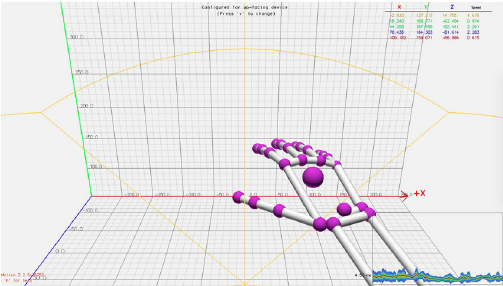
\includegraphics[width = .7\linewidth]{pic/1.png}
    \caption{Visualization of arm robot}
    \label{fig:fig1}
\end{figure}
\begin{figure}[h]
    \centering
    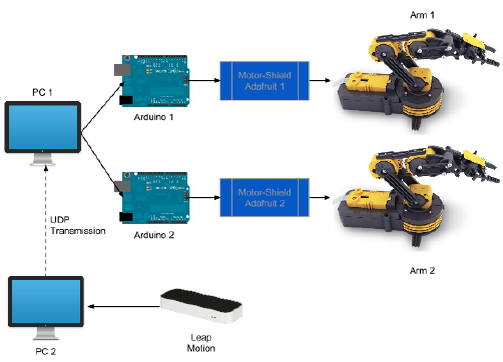
\includegraphics[width = .75\linewidth]{pic/5.png}
    \caption{Hardware architecture of arm robot}
    \label{fig:fig2}
\end{figure}
The proposed solution will address several challenges faced by the current industrial landscape, including the need for increased efficiency and productivity, the need for flexibility in the tasks performed by robotic arms, and the need for a more user-friendly control system. The expected outcome of this project is a versatile and reliable robotic arm that can perform a wide range of tasks with high accuracy and dexterity, and a control system that is easy to use and can be integrated with other systems.\\
So I am thinking that the machine I am going to make will be better then the robots recently made. My robot will be made based on comparatively easier algorithms. So the operation to be done by my robot may be faster. The design of the arm of my robot is visualized if figure~\ref{fig:fig1}. The component I am thinking to use to make the robot will not be much expensive and low quality. I will use high quality and well-designed hardware components for making the robot. The hardware architecture operated remotely is shown in figure~\ref{fig:fig2}. The robot may be less weight so it will consume less power.\\
The  movement  of  the  hands  and  fingers  of  the  user  is captured, in real time at a  frequency  of  120  fps, through only one Leap  Motion  device ~\cite{Motion}. Then,  a  computer  processes  this information.  If  the user  generates  a  gesture  or  places a  hand over a  limit,  it  triggers  a  command and sends  it  to  one of  the two  Arduino  that  serve  as  controllers  of  both  robotic  arms (each  Arduino  related  to  a  specific  arm).  Each  Arduino  is attached  to an  Adafruit  Motor-Shield \cite{Shield}  that  sends  electrical signals to  an  Owi robotic arm that  can be  moved according to the user's movements.\\
This project will provide valuable experience and knowledge in the design and development of robotic arms, control systems, and user interfaces, and will contribute to the advancement of automation in various industrial sectors.\\